%% Time-stamp: <2019-01-22 14:47:04 (marc)>
\documentclass[xcolor=x11names,compress, mathserif]{beamer}

\newcommand\hmmax{0}
\newcommand\bmmax{0}

\usepackage{../includes/MarkMathCmds}

\newcommand{\hackspace}{\hspace{4.2mm}}
\newcommand{\showstudent}[1]{}




% talk/author information
\newcommand{\authorname}{Mark van der Wilk}
\newcommand{\authoremail}{m.vdwilk@imperial.ac.uk}
\newcommand{\authoraffiliation}{
 Department of Computing\\Imperial
  College London}
\newcommand{\authortwitter}{markvanderwilk}
\newcommand{\slidesettitle}{\imperialBlue{From Linear Models \\ to Gaussian Processes}}
\newcommand{\footertitle}{From Linear Models to GPs}
\newcommand{\location}{Imperial College London}
\newcommand{\talkDate}{{January 23, 2023}}





\date{\imperialGray{\talkDate}}




% load defaults
\selectcolormodel{rgb}
\usepackage{ifxetex,ifluatex}
\newif\ifxetexorluatex
\ifxetex
  \xetexorluatextrue
\else
  \ifluatex
    \xetexorluatextrue
  \else
    \xetexorluatexfalse
  \fi
\fi

\usepackage{textpos}
%\usepackage{arabtex}
\usepackage{tikz}
\usetikzlibrary{decorations.markings}
\usetikzlibrary{arrows}
\usetikzlibrary{shapes}
\usetikzlibrary{plotmarks}
\usetikzlibrary{mindmap,trees,backgrounds}

\tikzstyle{every picture}+=[remember picture]

%\usepackage{movie15}
% \usepackage{pdfpages}
%\usepackage{xmpmulti}

\usepackage{anyfontsize}
\usepackage{wrapfig}
\usepackage{animate}
\usepackage{multirow}
\usepackage{multimedia}
\usepackage{xmpmulti}
%\usepackage[latin9]{inputenc}
\usepackage[english]{babel}
\usepackage{scalefnt}
\usepackage{verbatim}
\usepackage{url}
% \usepackage{pgf,pgfarrows,pgfnodes}
\usepackage{textpos}
\usepackage[tight,ugly]{units}
\usepackage{url}
\usepackage{bbm}
\usepackage[english]{babel}
\usepackage{fancyhdr}
\usepackage{bm} % correct bold symbols, like \bm
\usepackage{amsmath}
\usepackage{amsfonts}
\usepackage{amssymb}
\usepackage{mathrsfs}
\usepackage{mathtools}
\usepackage{color}
\usepackage{cancel}
\usepackage{algorithm}
\usepackage{algpseudocode}
\usepackage{mathrsfs}
\usepackage{listings}
\usepackage{graphicx} % for pdf, bitmapped graphics files
\usepackage{mathtools}
\usepackage{units}
\usepackage{subfig}
\usepackage{enumerate}
\usepackage{natbib}
\usepackage{dsfont}


\ifxetexorluatex
\usepackage{fontspec}
\setmainfont[Scale=0.8]{OpenDyslexic-Regular}
\else
\usefonttheme{professionalfonts}
\fi

\renewcommand{\vec}[1]{{\boldsymbol{{#1}}}} % vector
\newcommand{\mat}[1]{{\boldsymbol{{#1}}}} % matrix
% \newcommand{\KL}[2]{\mathrm{KL}(#1\|#2)} % KL divergence
\newcommand{\R}[0]{\mathds{R}} % real numbers
\newcommand{\Z}[0]{\mathds{Z}} % integers
\newcommand{\tr}[0]{\text{tr}} % trace
% \newcommand{\inv}{^{-1}}
% \DeclareMathOperator*{\diag}{diag}
\newcommand{\E}{\mathds{E}} % expectation
\newcommand{\var}{\mathds{V}}
\newcommand{\gauss}[2]{\mathcal{N}\big(#1,\,#2\big)}
\newcommand{\gaussx}[3]{\mathcal{N}\big(#1\,|\,#2,\,#3\big)}
\newcommand{\gaussBig}[2]{\mathcal{N}\left(#1,\,#2\right)}
\newcommand{\gaussxBig}[3]{\mathcal{N}\left(#1\,\left|\,#2,\,#3\right.\right)}
\newcommand{\Ber}[0]{\mathrm{Ber}} % Bernoulli distribution
\DeclareMathOperator{\cov}{Cov}
\ifxetexorluatex
\renewcommand{\T}[0]{^\top}
\renewcommand{\d}[0]{\text{d}} % derivative
\else
\newcommand{\T}[0]{^\top}
\renewcommand{\d}[0]{\text{d}} % derivative
\fi
% calculus
\newcommand{\pdiff}[1]{\frac{\partial}{\partial #1}}
\newcommand{\pdiffF}[2]{\frac{\partial #1}{\partial #2}}
\newcommand{\diffF}[2]{\frac{{\d}#1}{{\d}#2}}
\newcommand{\diffFII}[2]{\frac{{\d}^2 #1}{{\d}#2^2}}
\newcommand{\diff}[1]{\frac{{\d}}{{\d}#1}}
\newcommand{\diffII}[1]{\frac{{\d}^2}{{\d}#1^2}}
\newcommand{\class}[0]{\mathcal{C}}

\newcommand{\idx}[1]{^{(#1)}}
% \newcommand{\norm}[1]{\left\|#1\right\|}
\newcommand{\proj}[1]{\tilde{#1}}
\newcommand{\pcacoord}{z}
\newcommand{\pcacoordnew}{\zeta}
\newcommand{\latent}{z}
% \newcommand{\given}{\,|\,}
\newcommand{\genset}[1]{\mathrm{span}[#1]} % generating set
\newcommand{\set}[1]{\mathcal{#1}} % set
\newcommand{\fixgmfont}[1]{\scalebox{0.8}{#1}}



\usepackage{pifont}% http://ctan.org/pkg/pifont
\newcommand{\cmark}{{\color{green!40!black}\ding{51}}}%
\newcommand{\xmark}{{\color{red}\ding{55}}}%
\newcommand{\green}[1]{{\bf{\textcolor{green}{#1}}}}
\newcommand{\red}[1]{{\bf{\textcolor{red}{#1}}}}

\newcommand<>\red[1]{{\color#2[rgb]{1,0,0}#1}}
\newcommand<>\blue[1]{{\color#2[rgb]{0,0,1}#1}}
\newcommand<>\yellow[1]{{\color#2{camyellow}#1}}
\newcommand<>\green[1]{{\color#2[rgb]{0,0.6,0.0}#1}}
\newcommand<>\violet[1]{{\color#2[rgb]{0.6,0,0.6}#1}}
\newcommand<>\orange[1]{{\color#2[rgb]{1,0.5,0}#1}}
\newcommand<>\black[1]{{\color#2[rgb]{0,0,0}#1}}
\newcommand<>\steel[1]{{\color#2[rgb]{0,0,0.8}#1}}
\newcommand<>\darkblue[1]{{\color#2[rgb]{0,0,0.6}#1}}
\newcommand<>\lightblue[1]{{\color#2[rgb]{0.4,0.4,0.7}#1}}
\newcommand<>\gray[1]{{\color#2[rgb]{0.4,0.4,0.4}#1}}
\newcommand<>\greenish[1]{{\color#2[rgb]{0.45, 0.66, 0.45}#1}}
\newcommand<>\redish[1]{{\color#2[rgb]{0.7843    0.3706    0.3706}#1}}
\definecolor{redishTIKZ}{rgb}{0.7843, 0.3706, 0.3706}
\definecolor{imperialBlue}{rgb}{0.058, 0.219, 0.418}
\definecolor{aimsbrown}{rgb}{0.539, 0.117, 0.015}
% \definecolor{imperialGray}{rgb}{0.414, 0.488, 0.671 }
\definecolor{imperialGray}{RGB}{109,153, 204}
\definecolor{aimslightbrown}{RGB}{138,88,84}
\newcommand<>\imperialBlue[1]{{\color#2[rgb]{0.058, 0.219, 0.418}#1}}
\newcommand<>\aimsbrown[1]{{\color#2[rgb]{0.539, 0.117, 0.015}#1}}
%\newcommand<>\imperialGray[1]{{\color#2[rgb]{0.414, 0.488, 0.671}#1}}
\newcommand<>\imperialGray[1]{{\color#2[RGB]{109,153, 204}#1}}
\newcommand<>\aimslightbrown[1]{{\color#2[RGB]{138,88,84}#1}}
\newcommand<>\lightgray[1]{{\color#2[rgb]{0.8,0.8,0.8}#1}}
%\newcommand<>\highlightcolor[1]{{\color#2[rgb]{0,0,1}#1}}
\newcommand{\highlight}[1]{{\bf\steel{#1}}}
%\newcommand{\newblock}[0]{}

%\newcommand{\arrow}[0]{\includegraphics[height=5pt]{./figures/arrow}\hspace{3pt}}

\renewcommand{\emph}[1]{\textbf{\steel{{#1}}}}

\renewcommand{\alert}[1]{{\bf\red{{#1}}}}

\newcommand{\arrow}{
\begin{tikzpicture}
\draw [black!40!green, fill=black!40!green] (0,-0.12) -- (0,0.12) --
(0.15,0);
\draw [black!40!green, fill=black!40!green] (0.15,-0.12) -- (0.15,0.12) --
(0.3,0); 
\end{tikzpicture}
}

\geometry{left=0.45cm,top=0cm,right=0.45cm}


\newcommand{\logoimagepath}{./figures/imperial}
\newcommand{\highlightcolor}{blue!80!black}
%\newcommand{\headbarcolor}{imperialBlue}
\newcommand{\headbarcolor}{imperialBlue}
\institute{}

\newcommand{\coursetitle}{}

\newcommand{\slidesetsubtitle}{}
\newcommand{\slidesetnumber}{01}
\usefonttheme{professionalfonts}


\usetikzlibrary{decorations.fractals}
% tikzlibrary.code.tex
%
% Copyright 2010-2011 by Laura Dietz
% Copyright 2012 by Jaakko Luttinen
%
% The MIT License
%
% See LICENSE file for more details.

% Load other libraries
\usetikzlibrary{shapes}
\usetikzlibrary{fit}
\usetikzlibrary{chains}
\usetikzlibrary{arrows}

% Latent node
\tikzstyle{latent} = [circle,fill=white,draw=black,inner sep=1pt,
minimum size=20pt, font=\fontsize{10}{10}\selectfont, node distance=1]
% Observed node
\tikzstyle{obs} = [latent,fill=gray!25]
% Constant node
\tikzstyle{const} = [rectangle, inner sep=0pt, node distance=1]
% Factor node
\tikzstyle{factor} = [rectangle, fill=black,minimum size=5pt, inner
sep=0pt, node distance=0.4]
% Deterministic node
\tikzstyle{det} = [latent, diamond]

% Plate node
\tikzstyle{plate} = [draw, rectangle, rounded corners, fit=#1]
% Invisible wrapper node
\tikzstyle{wrap} = [inner sep=0pt, fit=#1]
% Gate
\tikzstyle{gate} = [draw, rectangle, dashed, fit=#1]

% Caption node
\tikzstyle{caption} = [font=\footnotesize, node distance=0] %
\tikzstyle{plate caption} = [caption, node distance=0, inner sep=0pt,
below left=5pt and 0pt of #1.south east] %
\tikzstyle{factor caption} = [caption] %
\tikzstyle{every label} += [caption] %

%\pgfdeclarelayer{b}
%\pgfdeclarelayer{f}
%\pgfsetlayers{b,main,f}

% \factoredge [options] {inputs} {factors} {outputs}
\newcommand{\factoredge}[4][]{ %
  % Connect all nodes #2 to all nodes #4 via all factors #3.
  \foreach \f in {#3} { %
    \foreach \x in {#2} { %
      \path (\x) edge[-,#1] (\f) ; %
      %\draw[-,#1] (\x) edge[-] (\f) ; %
    } ;
    \foreach \y in {#4} { %
      \path (\f) edge[->, >={triangle 45}, #1] (\y) ; %
      %\draw[->,#1] (\f) -- (\y) ; %
    } ;
  } ;
}

% \edge [options] {inputs} {outputs}
\newcommand{\edge}[3][]{ %
  % Connect all nodes #2 to all nodes #3.
  \foreach \x in {#2} { %
    \foreach \y in {#3} { %
      \path (\x) edge [->, >={triangle 45}, #1] (\y) ;%
      %\draw[->,#1] (\x) -- (\y) ;%
    } ;
  } ;
}

% \factor [options] {name} {caption} {inputs} {outputs}
\newcommand{\factor}[5][]{ %
  % Draw the factor node. Use alias to allow empty names.
  \node[factor, label={[name=#2-caption]#3}, name=#2, #1,
  alias=#2-alias] {} ; %
  % Connect all inputs to outputs via this factor
  \factoredge {#4} {#2-alias} {#5} ; %
}

% \plate [options] {name} {fitlist} {caption}
\newcommand{\plate}[4][]{ %
  \node[wrap=#3] (#2-wrap) {}; %
  \node[plate caption=#2-wrap] (#2-caption) {#4}; %
  \node[plate=(#2-wrap)(#2-caption), #1] (#2) {}; %
}

% \gate [options] {name} {fitlist} {inputs}
\newcommand{\gate}[4][]{ %
  \node[gate=#3, name=#2, #1, alias=#2-alias] {}; %
  \foreach \x in {#4} { %
    \draw [-*,thick] (\x) -- (#2-alias); %
  } ;%
}

% \vgate {name} {fitlist-left} {caption-left} {fitlist-right}
% {caption-right} {inputs}
\newcommand{\vgate}[6]{ %
  % Wrap the left and right parts
  \node[wrap=#2] (#1-left) {}; %
  \node[wrap=#4] (#1-right) {}; %
  % Draw the gate
  \node[gate=(#1-left)(#1-right)] (#1) {}; %
  % Add captions
  \node[caption, below left=of #1.north ] (#1-left-caption)
  {#3}; %
  \node[caption, below right=of #1.north ] (#1-right-caption)
  {#5}; %
  % Draw middle separation
  \draw [-, dashed] (#1.north) -- (#1.south); %
  % Draw inputs
  \foreach \x in {#6} { %
    \draw [-*,thick] (\x) -- (#1); %
  } ;%
}

% \hgate {name} {fitlist-top} {caption-top} {fitlist-bottom}
% {caption-bottom} {inputs}
\newcommand{\hgate}[6]{ %
  % Wrap the left and right parts
  \node[wrap=#2] (#1-top) {}; %
  \node[wrap=#4] (#1-bottom) {}; %
  % Draw the gate
  \node[gate=(#1-top)(#1-bottom)] (#1) {}; %
  % Add captions
  \node[caption, above right=of #1.west ] (#1-top-caption)
  {#3}; %
  \node[caption, below right=of #1.west ] (#1-bottom-caption)
  {#5}; %
  % Draw middle separation
  \draw [-, dashed] (#1.west) -- (#1.east); %
  % Draw inputs
  \foreach \x in {#6} { %
    \draw [-*,thick] (\x) -- (#1); %
  } ;%
}


% Copyright (C) 2016  Joseph Rabinoff

% ipe2tikz is free software; you can redistribute it and/or modify it under
% the terms of the GNU General Public License as published by the Free
% Software Foundation; either version 3 of the License, or (at your option)
% any later version.

% ipe2tikz is distributed in the hope that it will be useful, but WITHOUT ANY
% WARRANTY; without even the implied warranty of MERCHANTABILITY or FITNESS
% FOR A PARTICULAR PURPOSE.  See the GNU General Public License for more
% details.

% You should have received a copy of the GNU General Public License along with
% ipe2tikz; if not, you can find it at "http://www.gnu.org/copyleft/gpl.html",
% or write to the Free Software Foundation, Inc., 675 Mass Ave, Cambridge, MA
% 02139, USA.


% ipe compatibility TikZ styles

\usetikzlibrary{arrows.meta}

\makeatletter

% These should behave almost exactly like ipe arrows.  They disable correcting
% for the miter length and line width.  This is important for visual consistency
% with ipe, since ipe arrows get much larger when the line width is increased.
% They also use the line join and cap styles from the main path.  These are very
% simple arrows: there is no harpoon version, and the convex hull computation is
% sloppy.

\pgfdeclarearrow{
  name = ipe _linear,
  defaults = {
    length = +1bp,
    width  = +.666bp,
    line width = +0pt 1,
  },
  setup code = {
    % Control points
    \pgfarrowssetbackend{0pt}
    \pgfarrowssetvisualbackend{
      \pgfarrowlength\advance\pgf@x by-.5\pgfarrowlinewidth}
    \pgfarrowssetlineend{\pgfarrowlength}
    \ifpgfarrowreversed
      \pgfarrowssetlineend{\pgfarrowlength\advance\pgf@x by-.5\pgfarrowlinewidth}
    \fi
    \pgfarrowssettipend{\pgfarrowlength}
    % Convex hull
    \pgfarrowshullpoint{\pgfarrowlength}{0pt}
    \pgfarrowsupperhullpoint{0pt}{.5\pgfarrowwidth}
    % The following are needed in the code:
    \pgfarrowssavethe\pgfarrowlinewidth
    \pgfarrowssavethe\pgfarrowlength
    \pgfarrowssavethe\pgfarrowwidth
  },
  drawing code = {
    \pgfsetdash{}{+0pt}
    \ifdim\pgfarrowlinewidth=\pgflinewidth\else\pgfsetlinewidth{+\pgfarrowlinewidth}\fi
    \pgfpathmoveto{\pgfqpoint{0pt}{.5\pgfarrowwidth}}
    \pgfpathlineto{\pgfqpoint{\pgfarrowlength}{0pt}}
    \pgfpathlineto{\pgfqpoint{0pt}{-.5\pgfarrowwidth}}
    \pgfusepathqstroke
  },
  parameters = {
    \the\pgfarrowlinewidth,%
    \the\pgfarrowlength,%
    \the\pgfarrowwidth,%
  },
}


\pgfdeclarearrow{
  name = ipe _pointed,
  defaults = {
    length = +1bp,
    width  = +.666bp,
    inset  = +.2bp,
    line width = +0pt 1,
  },
  setup code = {
    % Control points
    \pgfarrowssetbackend{0pt}
    \pgfarrowssetvisualbackend{\pgfarrowinset}
    \pgfarrowssetlineend{\pgfarrowinset}
    \ifpgfarrowreversed
      \pgfarrowssetlineend{\pgfarrowlength}
    \fi
    \pgfarrowssettipend{\pgfarrowlength}
    % Convex hull
    \pgfarrowshullpoint{\pgfarrowlength}{0pt}
    \pgfarrowsupperhullpoint{0pt}{.5\pgfarrowwidth}
    \pgfarrowshullpoint{\pgfarrowinset}{0pt}
    % The following are needed in the code:
    \pgfarrowssavethe\pgfarrowinset
    \pgfarrowssavethe\pgfarrowlinewidth
    \pgfarrowssavethe\pgfarrowlength
    \pgfarrowssavethe\pgfarrowwidth
  },
  drawing code = {
    \pgfsetdash{}{+0pt}
    \ifdim\pgfarrowlinewidth=\pgflinewidth\else\pgfsetlinewidth{+\pgfarrowlinewidth}\fi
    \pgfpathmoveto{\pgfqpoint{\pgfarrowlength}{0pt}}
    \pgfpathlineto{\pgfqpoint{0pt}{.5\pgfarrowwidth}}
    \pgfpathlineto{\pgfqpoint{\pgfarrowinset}{0pt}}
    \pgfpathlineto{\pgfqpoint{0pt}{-.5\pgfarrowwidth}}
    \pgfpathclose
    \ifpgfarrowopen
      \pgfusepathqstroke
    \else
      \ifdim\pgfarrowlinewidth>0pt\pgfusepathqfillstroke\else\pgfusepathqfill\fi
    \fi
  },
  parameters = {
    \the\pgfarrowlinewidth,%
    \the\pgfarrowlength,%
    \the\pgfarrowwidth,%
    \the\pgfarrowinset,%
    \ifpgfarrowopen o\fi%
  },
}


% For correcting minipage width in stretched nodes
\newdimen\ipeminipagewidth
\def\ipestretchwidth#1{%
  \pgfmathsetlength{\ipeminipagewidth}{#1/\ipenodestretch}}

\tikzstyle{ipe import} = [
  % General ipe defaults
  x=1bp, y=1bp,
%
  % Nodes
  ipe node stretch/.store in=\ipenodestretch,
  ipe stretch normal/.style={ipe node stretch=1},
  ipe stretch normal,
  ipe node/.style={
    anchor=base west, inner sep=0, outer sep=0, scale=\ipenodestretch
  },
%
  % Use a special key for the mark scale, so that the default can be overriden.
  % (This doesn't happen with the scale= key; those accumulate.)
  ipe mark scale/.store in=\ipemarkscale,
%
  ipe mark tiny/.style={ipe mark scale=1.1},
  ipe mark small/.style={ipe mark scale=2},
  ipe mark normal/.style={ipe mark scale=3},
  ipe mark large/.style={ipe mark scale=5},
%
  ipe mark normal, % Set default
%
  ipe circle/.pic={
    \draw[line width=0.2*\ipemarkscale]
      (0,0) circle[radius=0.5*\ipemarkscale];
    \coordinate () at (0,0);
  },
  ipe disk/.pic={
    \fill (0,0) circle[radius=0.6*\ipemarkscale];
    \coordinate () at (0,0);
  },
  ipe fdisk/.pic={
    \filldraw[line width=0.2*\ipemarkscale]
      (0,0) circle[radius=0.5*\ipemarkscale];
    \coordinate () at (0,0);
  },
  ipe box/.pic={
    \draw[line width=0.2*\ipemarkscale, line join=miter]
      (-.5*\ipemarkscale,-.5*\ipemarkscale) rectangle
      ( .5*\ipemarkscale, .5*\ipemarkscale);
    \coordinate () at (0,0);
  },
  ipe square/.pic={
    \fill
      (-.6*\ipemarkscale,-.6*\ipemarkscale) rectangle
      ( .6*\ipemarkscale, .6*\ipemarkscale);
    \coordinate () at (0,0);
  },
  ipe fsquare/.pic={
    \filldraw[line width=0.2*\ipemarkscale, line join=miter]
      (-.5*\ipemarkscale,-.5*\ipemarkscale) rectangle
      ( .5*\ipemarkscale, .5*\ipemarkscale);
    \coordinate () at (0,0);
  },
  ipe cross/.pic={
    \draw[line width=0.2*\ipemarkscale, line cap=butt]
      (-.5*\ipemarkscale,-.5*\ipemarkscale) --
      ( .5*\ipemarkscale, .5*\ipemarkscale)
      (-.5*\ipemarkscale, .5*\ipemarkscale) --
      ( .5*\ipemarkscale,-.5*\ipemarkscale);
    \coordinate () at (0,0);
  },
%
  % Arrow sizes (for TikZ arrows)
  /pgf/arrow keys/.cd,
  ipe arrow normal/.style={scale=1},
  ipe arrow tiny/.style={scale=.4},
  ipe arrow small/.style={scale=.7},
  ipe arrow large/.style={scale=1.4},
  ipe arrow normal,
  /tikz/.cd,
%
  % Approximations to ipe arrows
  % Put in a style to allow to reset default scale when "ipe arrow normal" is
  % changed.  I think this is the only way, since all the parameters to arrows
  % are expanded when the tip is declared.
  ipe arrows/.style={
    ipe normal/.tip={
      ipe _pointed[length=1bp, width=.666bp, inset=0bp,
                   quick, ipe arrow normal]},
    ipe pointed/.tip={
      ipe _pointed[length=1bp, width=.666bp, inset=0.2bp,
                   quick, ipe arrow normal]},
    ipe linear/.tip={
      ipe _linear[length = 1bp, width=.666bp,
                  ipe arrow normal, quick]},
    ipe fnormal/.tip={ipe normal[fill=white]},
    ipe fpointed/.tip={ipe pointed[fill=white]},
    ipe double/.tip={ipe normal[] ipe normal},
    ipe fdouble/.tip={ipe fnormal[] ipe fnormal},
    % These should maybe use [bend], but that often looks bad unless it's on an
    % actual arc.
    ipe arc/.tip={ipe normal},
    ipe farc/.tip={ipe fnormal},
    ipe ptarc/.tip={ipe pointed},
    ipe fptarc/.tip={ipe fpointed},
  },
  ipe arrows, % Set default sizes
]

% I'm not sure how to do this in a .style, since the #args get confused.
\tikzset{
  rgb color/.code args={#1=#2}{%
    \definecolor{tempcolor-#1}{rgb}{#2}%
    \tikzset{#1=tempcolor-#1}%
  },
}

\makeatother

\endinput

\usetikzlibrary{matrix,positioning,decorations.pathreplacing}
\usetikzlibrary{calc,quotes,angles}
\usetikzlibrary{arrows, arrows.meta, patterns}

\usetikzlibrary{decorations.pathreplacing}
\tikzset{
    position label/.style={
       above = 3pt,
       text height = 2ex,
       text depth = 1ex
    }
}

% \usetikzlibrary{decorations.markings}
\tikzset{
  font={\fontsize{14pt}{12}\selectfont}
}



\useoutertheme[subsection=false,shadow]{miniframes}
\useinnertheme{default}
\usefonttheme{serif}
%\usepackage{palatino}
\usepackage{mathpazo}
%\usepackage{utopia}
\usepackage{stmaryrd} % for varodot, bigodot 
\usepackage{mathabx} % for \coAsterisk
%\usepackage{mnsymbol}
%\setbeamertemplate{itemize item}{\scriptsize\raise1.7pt\hbox{\donotcoloroutermaths$\Asterisk$}}
%\setbeamertemplate{itemize item}{\scriptsize\raise1.7pt\hbox{\donotcoloroutermaths$\varodot$}}
%\setbeamertemplate{itemize subitem}{\scriptsize\raise1.25pt\hbox{\donotcoloroutermaths$\rhd$}}

\usepackage{xifthen}% provides \isempty tesst

\setbeamerfont{title like}{shape=\scshape}
\setbeamerfont{frametitle}{}



\setbeamercolor*{lower separation line head}{bg=blue} 
\setbeamercolor*{normal text}{fg=black,bg=white} 
\setbeamercolor*{alerted text}{fg=red} 
\setbeamercolor*{example text}{fg=black} 
%\setbeamercolor*{frametitle}{fg=aimsbrown} 
\setbeamercolor*{frametitle}{fg=imperialBlue} 
\setbeamercolor*{structure}{fg=black} 
 
\setbeamercolor*{palette tertiary}{fg=black,bg=black!10} 
\setbeamercolor*{palette quaternary}{fg=black,bg=black!10} 

%\renewcommand{\(}{\begin{columns}}
%\renewcommand{\)}{\end{columns}}
%\newcommand{\<}[1]{\begin{column}{#1}}
%\renewcommand{\>}{\end{column}}

% ======================================
% custom commands 
\newcommand{\cemph}[1]{\textcolor{\highlightcolor}{#1}}
\newcommand{\calert}[1]{\textcolor{red}{#1}}

\setbeamertemplate{navigation symbols}{}
%\renewcommand\frametitle[1]{{\textsc{\Large \textcolor{\highlightcolor}{#1}}}\vspace{0.6cm}\par}

\setbeamertemplate{frametitle}
{
{\textsc\bf \insertframetitle}\vspace{0.2cm}\par
}


%%%%%%%%%%%%%%%%%%%%%%%%%%%%%%%%%%%%%%%%%%%%%%%%%%
\setbeamertemplate{headline}{% 
	\setbeamercolor{head1}{bg=\headbarcolor}
	 \hbox{%
  \begin{beamercolorbox}[wd=.01\paperwidth,ht=2.25ex,dp=50ex,center]{head1}%
  \fontsize{5}{5}\selectfont  
  \end{beamercolorbox}%
  }
  \vspace{-50ex}
}
\setbeamertemplate{footline}{
\begin{tiny}
\setbeamercolor{foot1}{fg=black,bg=gray!10}
\setbeamercolor{foot2}{fg=gray,bg=gray!15}
\setbeamercolor{foot3}{fg=gray,bg=gray!10}
\setbeamercolor{foot4}{fg=black,bg=gray!20}
\setbeamercolor{foot5}{fg=gray,bg=gray!15}
\setbeamercolor{foot6}{fg=black,bg=gray!20}

% taken from theme infolines and adapted
  \leavevmode%
  \hbox{%
  \begin{beamercolorbox}[wd=.45\paperwidth,ht=2.25ex,dp=1ex,center]{foot1}%
  \fontsize{5}{5}\selectfont
  \flushleft \hspace*{2ex}{\footertitle}
  \end{beamercolorbox}%
  % \begin{beamercolorbox}[wd=.08\paperwidth,ht=2.25ex,dp=1ex,center]{foot2}
  % \end{beamercolorbox}%
  %   \begin{beamercolorbox}[wd=.05\paperwidth,ht=2.25ex,dp=1ex,center]{foot3}
  % \end{beamercolorbox}%
    \begin{beamercolorbox}[wd=.45\paperwidth,ht=2.25ex,dp=1ex,center]{foot4}%
  \fontsize{5}{5}\selectfont
  \authorname\hspace{5mm}@\location, \talkDate%\ (\authorweb) 
  \end{beamercolorbox}%
  % \begin{beamercolorbox}[wd=.05\paperwidth,ht=2.25ex,dp=1ex,center]{foot5}
  % \end{beamercolorbox}%
  \begin{beamercolorbox}[wd=.1\paperwidth,ht=2.25ex,dp=1ex,right]{foot6}%
	\insertframenumber{}  \hspace*{2ex} 
  \end{beamercolorbox}}%
  \vskip0pt%
\end{tiny}
\vskip0pt
}


\setbeamercolor{block title}{bg=imperialBlue!45, fg=white}
\setbeamertemplate{blocks}[rounded][shadow=true]


\newenvironment<>{myblock}[1]{%
  \begin{actionenv}#2%
      \def\insertblocktitle{#1}%
      \par%
      \mode<presentation>{%
%       \setbeamercolor{block title}{fg=black,bg=aimslightbrown!50!white}
      \setbeamercolor{block title}{fg=black,bg=imperialBlue!45!white}
       \setbeamercolor{block body}{fg=black,bg=gray!20}
       \setbeamercolor{itemize item}{fg=blue!40!white}
       \setbeamertemplate{itemize item}[triangle]
     }%
      \usebeamertemplate{block begin}}
    {\par\usebeamertemplate{block end}\end{actionenv}}

\newenvironment<>{myblock2}[1]{%
  \begin{actionenv}#2%
      \def\insertblocktitle{#1}%
      \par%
      \mode<presentation>{%
       \setbeamercolor{block title}{fg=white,bg=blue!80!black}
       \setbeamercolor{block body}{fg=black,bg=gray!20}
       \setbeamercolor{itemize item}{fg=green!60!black}
       \setbeamertemplate{itemize item}[triangle]
     }%
      \usebeamertemplate{block begin}}
    {\par\usebeamertemplate{block end}\end{actionenv}}

\gdef\colchar#1#2{%
  \tikz[baseline]{%
%  \node[anchor=base,inner sep=2pt,outer sep=0pt,fill = #2!20]
%  {\large{#1}};
  \node[anchor=base,inner sep=1pt,outer sep=0pt,fill = #2!20]
  {{\fontsize{11}{13}\selectfont #1}};
    }%
}%
\gdef\drawfontframe#1#2{%
  \tikz[baseline]{%
  \node[anchor=base,inner sep=2pt,outer sep=0pt,fill = #2!20] {#1};
    }%
  }%


\makeatletter
\let\@@magyar@captionfix\relax
\makeatother

%%% Local Variables:
%%% mode: latex
%%% TeX-master: "2018-09-arusha-linear-regression"
%%% End:



\newif\iflattersubsect

\AtBeginSection[] {
    \begin{frame}<beamer>
    \frametitle{Overview} %
    \tableofcontents[currentsection]  
    \end{frame}
    \lattersubsectfalse
}

\AtBeginSubsection[] {
    \iflattersubsect
    \begin{frame}<Coming Next>
    \frametitle{Overview} %
    \tableofcontents[currentsubsection]  
    \end{frame}
    \fi
    \lattersubsecttrue
}

\begin{document}


%%%%%%%%%%%%%%%%%%%%%%%%%%%%%%%%%%%%%%%%%%%%%%%%%%%%%%

{\setbeamertemplate{footline}{}
\begin{frame}
\title{\slidesettitle}
%\subtitle{SUBTITLE}
\author{\footnotesize
  \textbf{\authorname}
 }

 %%% LOGO

% \begin{flushright}
%   % \begin{columns}
%   %   \column{0.5\hsize}
%   %   \column{0.45\hsize}
%
\includegraphics[height = 8mm]{./figures/qla}\hspace{2mm}
%     
\includegraphics[height = 8mm]{./figures/aims-rwanda}\\[2mm]
%
\includegraphics[height = 8mm]{./figures/imperial}
%%\end{columns}
%\end{flushright}

\vspace{-0cm}
%\begin{flushleft}
%\vspace{-1.5cm}{\small \textcolor{blue}{\coursetitle}}\\\vspace{2cm}
{\huge \slidesettitle \ifthenelse{\equal{\slidesetsubtitle}{}}%
    {}% if #1 is empty
    {: \\ {\large \slidesetsubtitle}}% if #1 is not empty
    } \\    
    %\vspace{20pt}
%\end{flushleft}
  
 
% this is all stuff below the talk title. make two columns, just in
% case you want to have a picture or a second affiliation here 
\begin{columns}[t]
\column{0.8\hsize}
%\begin{flushleft}
\begin{columns}[t]
\column{0.6\hsize}
\insertauthor \\[2mm]
\authoraffiliation\\[2mm]
\column{0.25\hsize}
\\[2mm]

\includegraphics[height = 0.3cm]{./figures/twitter}{\small @\authortwitter}\\[-1mm]
\mbox{\small \url{\authoremail}}
\end{columns}
\column{0.14\hsize}
\end{columns}
% \authorweb\\
\vspace{7mm}
% \aimslightbrown{The Nelson Mandela African Institute of Science and
%   Technology\\Arusha, Tanzania}\\[2mm]
\insertdate
%\end{flushleft}
\end{frame}
}

%%% Local Variables:
%%% mode: latex
%%% TeX-master: t
%%% End:


\begin{frame}{Recap}
Last lecture we saw that:
\begin{itemize}
\item The prior has a large effect on the predictions \& we needed a sensible prior.
\item Polynomial bases didn't lead to a sensible prior, squared exponential did.
\item We needed many basis functions to ensure sensible uncertainty.
\end{itemize}
\begin{overprint}
\begin{figure}
\centering
\onslide*<1>{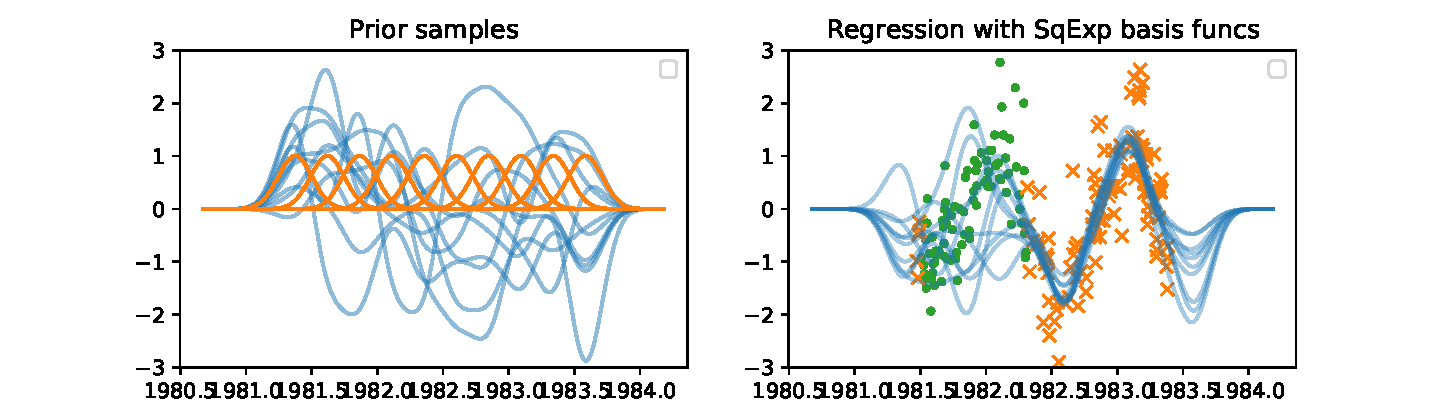
\includegraphics[width=\hsize,trim=2.2cm 0 2.2cm 0,clip]{./figures/gp/regression_basisfunc_prior_post_samples.pdf}}
\onslide*<2>{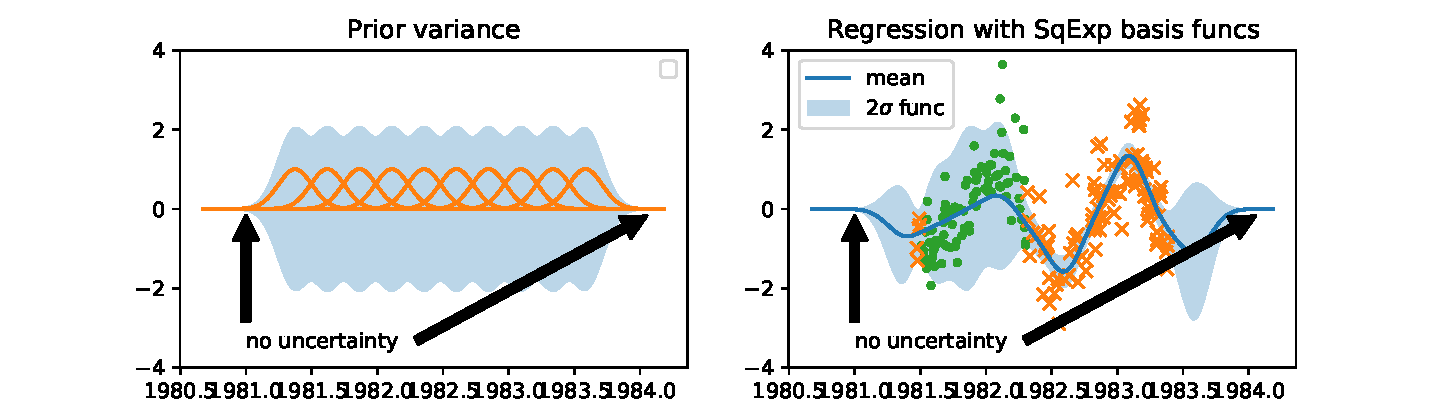
\includegraphics[width=\hsize,trim=2.2cm 0 2.2cm 0,clip]{./figures/gp/regression_basisfunc_prior_post.pdf}}
\onslide*<3>{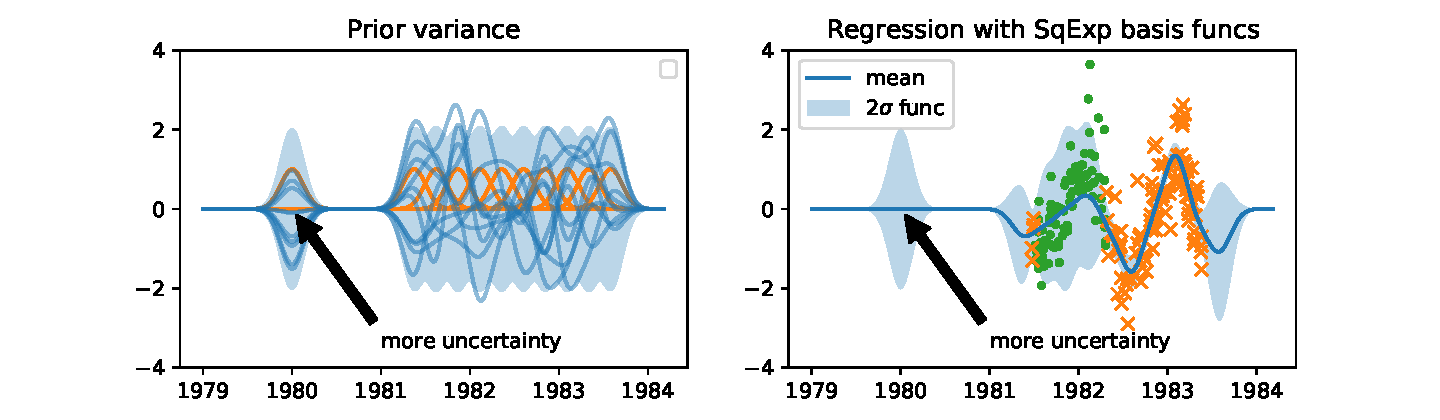
\includegraphics[width=\hsize,trim=2.2cm 0 2.2cm 0,clip]{./figures/gp/regression_basisfunc_prior_post_extrabasis.pdf}}
\onslide*<4>{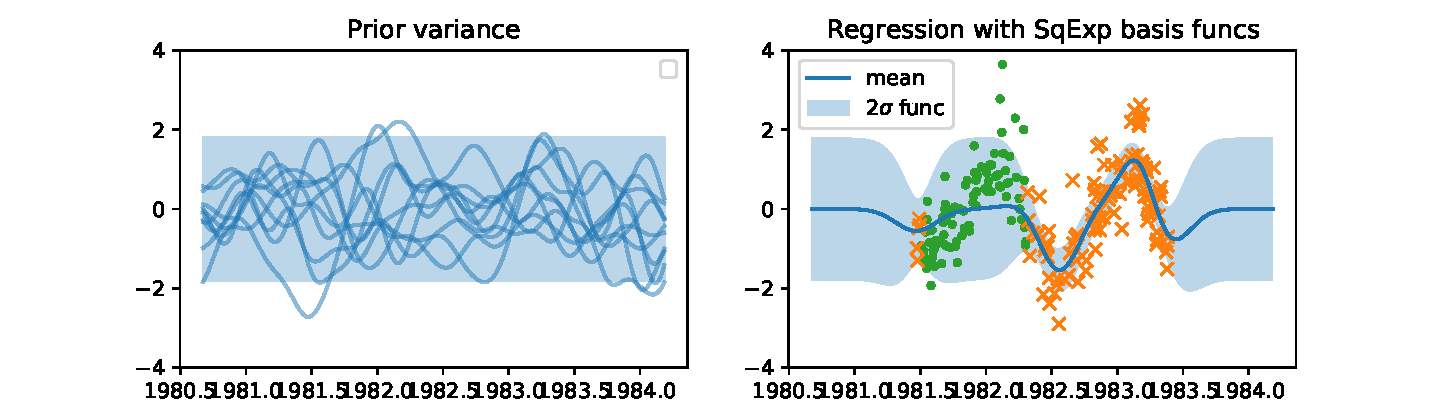
\includegraphics[width=\hsize,trim=2.2cm 0 2.2cm 0,clip]{./figures/gp/regression_basisfunc_prior_post_infinitebasis.pdf}}
\end{figure}
\end{overprint}
\end{frame}


\begin{frame}{Today}
We will see:
\begin{itemize}
\item By considering computational cost, we derive the Gaussian process view of BLR.
\item This is the kernel trick!
\item What is a Gaussian process.
\item How to find posteriors in GP models.
\end{itemize}
\end{frame}


\begin{frame}{Infinite Basis Functions: Another Reason}
\begin{overprint}
\onslide*<1>{\begin{figure}\centering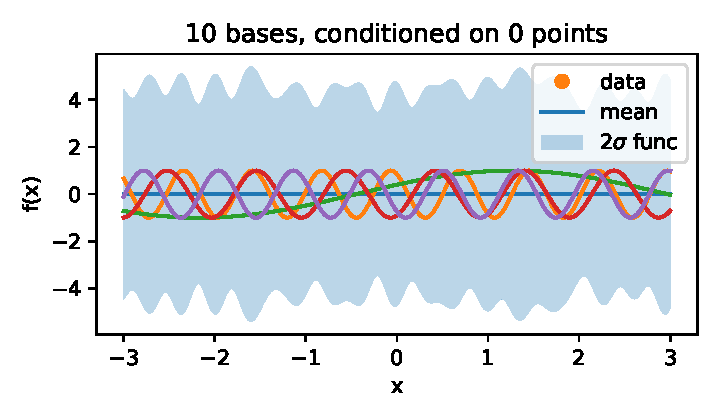
\includegraphics[width=0.7\hsize]{./figures/gp/regression_basisfunc_add_data0.pdf}\end{figure}}
\onslide*<2>{\begin{figure}\centering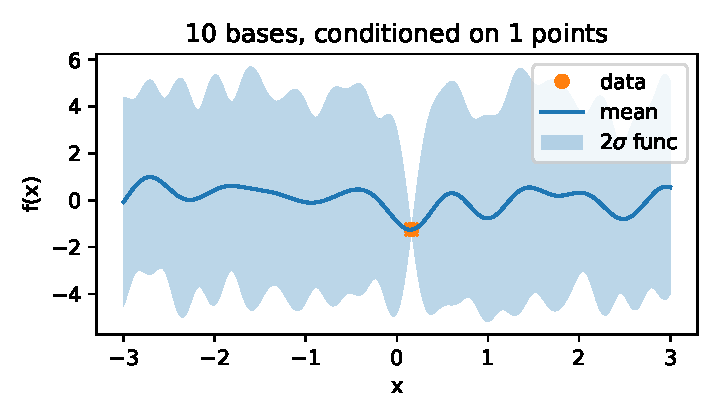
\includegraphics[width=0.7\hsize]{./figures/gp/regression_basisfunc_add_data1.pdf}\end{figure}}
\onslide*<3>{\begin{figure}\centering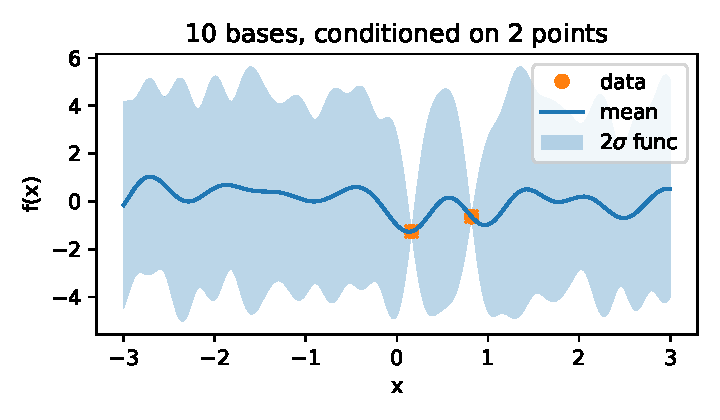
\includegraphics[width=0.7\hsize]{./figures/gp/regression_basisfunc_add_data2.pdf}\end{figure}}
\onslide*<4>{\begin{figure}\centering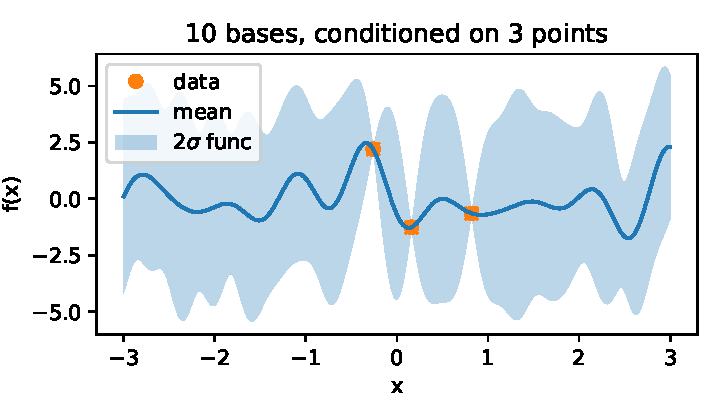
\includegraphics[width=0.7\hsize]{./figures/gp/regression_basisfunc_add_data3.pdf}\end{figure}}
\onslide*<5>{\begin{figure}\centering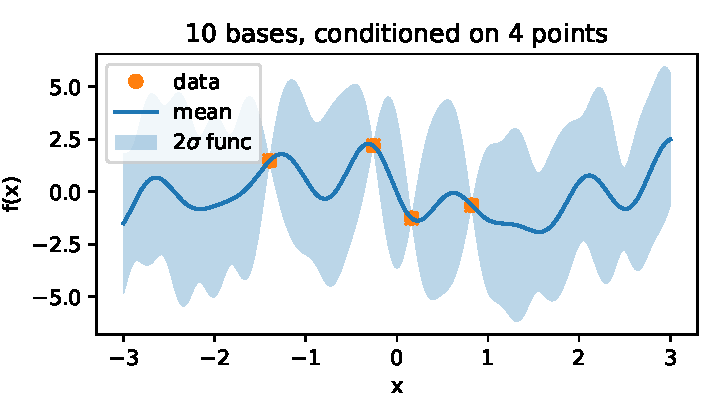
\includegraphics[width=0.7\hsize]{./figures/gp/regression_basisfunc_add_data4.pdf}\end{figure}}
\onslide*<6>{\begin{figure}\centering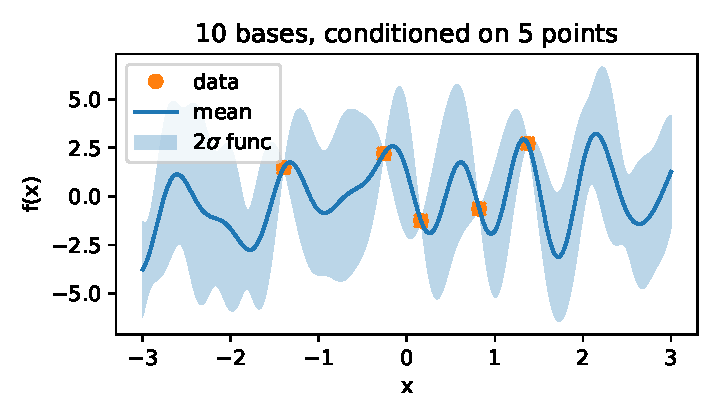
\includegraphics[width=0.7\hsize]{./figures/gp/regression_basisfunc_add_data5.pdf}\end{figure}}
\onslide*<7>{\begin{figure}\centering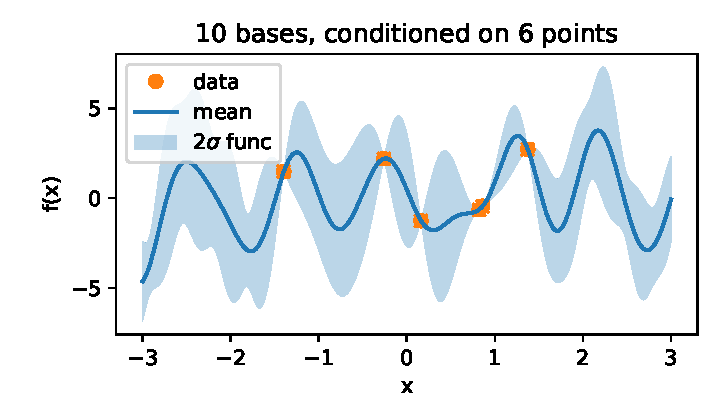
\includegraphics[width=0.7\hsize]{./figures/gp/regression_basisfunc_add_data6.pdf}\end{figure}}
\onslide*<8>{\begin{figure}\centering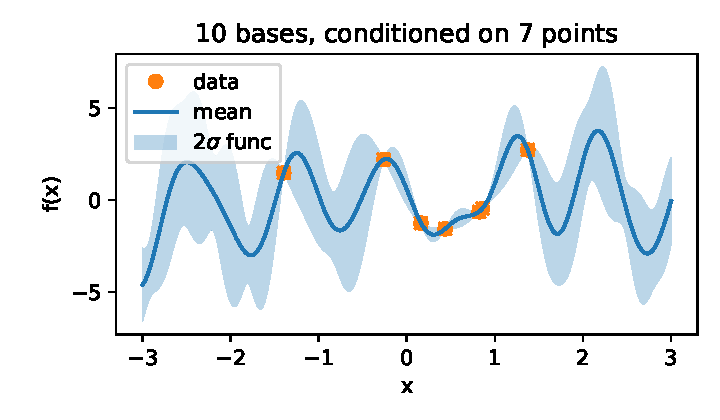
\includegraphics[width=0.7\hsize]{./figures/gp/regression_basisfunc_add_data7.pdf}\end{figure}}
\onslide*<9>{\begin{figure}\centering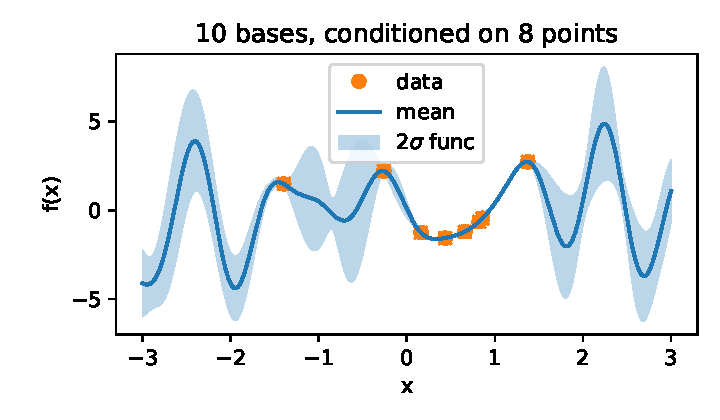
\includegraphics[width=0.7\hsize]{./figures/gp/regression_basisfunc_add_data8.pdf}\end{figure}}
\onslide*<10>{\begin{figure}\centering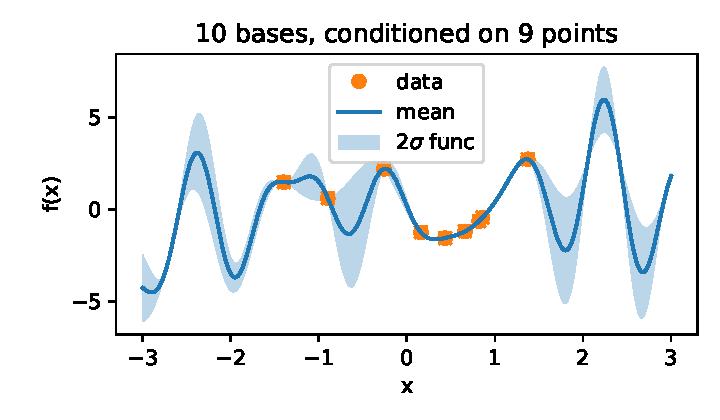
\includegraphics[width=0.7\hsize]{./figures/gp/regression_basisfunc_add_data9.pdf}\end{figure}}
\onslide*<11->{\begin{figure}\centering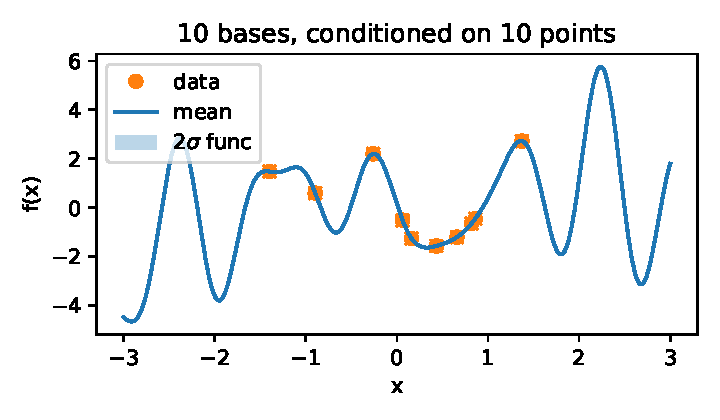
\includegraphics[width=0.7\hsize]{./figures/gp/regression_basisfunc_add_data10.pdf}\end{figure}}
\end{overprint}

\vspace{-0.5cm}
\begin{itemize}
\item Non-local basis functions give uncertainty everywhere (like polynomials).
\item But uncertainty decreases non-locally!
\item For $M$ bases, when we condition on $M$ points: full certainty!
\end{itemize}
\uncover<12>{\scriptsize \emph{Exercise:} For a model with $M$ bases, show that after conditioning on $M$ points (zero variance likelihood) leads to 1) completely certain predictions, 2) certain posterior.}
\end{frame}


\begin{frame}{BLR: Computing the Posterior}
For Gaussian models, finding conditionals can easily be done by finding the \emph{joint}, and then applying the \emph{Gaussian conditioning rule}.
\begin{gather}
\vtheta \sim \NormDist{0, \mat I_M}\,, \qquad \vepsilon \sim \NormDist{0, \mat I_N\sigma^2}\,, \qquad [\Phi(\mat X)]_{nm} = \phi_m(\vx_n) \,. \\
\vtheta \in \Reals^M\,,\quad \vy \in \Reals^N \,,\quad \vepsilon \in \Reals^N\,,\quad \Phi(\mat X) \in \Reals^{N\times M}\,,\quad \mat X \in \Reals^{N\times D}\,.
\end{gather}
\vspace{-0.4cm}
\begin{align}
\begin{bmatrix}
\vtheta \\
\vy
\end{bmatrix} &= 
\begin{bmatrix}
\mat I_M & 0 \\
\Phi(\mat X) & \mat I_n
\end{bmatrix}\begin{bmatrix}
\vtheta \\ \vepsilon
\end{bmatrix}\\
\implies p\left(\begin{bmatrix}\vtheta \\ \vy\end{bmatrix}\right) &= \NormDist{\begin{bmatrix}\vtheta \\ \vy \end{bmatrix};
0, \begin{bmatrix}
\mat I_M & \Phi(\mat X)\transpose \\
\Phi(\mat X) & \Phi(\mat X)\Phi(\mat X)\transpose + \sigma^2\mat I_N
\end{bmatrix}}
\end{align}
Using:
\begin{itemize}
\item Linear relationships between Gaussian RVs gives Gaussian joint.
\begin{itemize}
  \item Write joint Gaussian as a linear transformation of RVs \cemph{with known independent distributions}.
\end{itemize}
\item $\Exp{\NormDist{\vx; \vmu, \mat\Sigma}}{\mat A\vx} = \mat A\vmu$, and $\Var{\NormDist{\vx; \vmu, \mat\Sigma}}{\mat A\vx} = \mat A\mat\Sigma\mat A\transpose$.
\end{itemize}
\end{frame}


\begin{frame}{BLR: Computing the Posterior}
Gaussian conditioning formula (will be provided in exam):
\begin{align}
p\left(\begin{bmatrix}\vx_1 \\ \vx_2\end{bmatrix}\right) &= \NormDist{\begin{bmatrix}\vx_1 \\ \vx_2 \end{bmatrix};
\begin{bmatrix}\vmu_1 \\ \vmu_2\end{bmatrix}, \begin{bmatrix}
\mat\Sigma_{11} & \mat\Sigma_{12} \\
\mat\Sigma_{21} & \mat\Sigma_{22}\end{bmatrix}} \\
p(\vx_2|\vx_1) &= \NormDist{\vx_2; \vmu_2 + \mat\Sigma_{21}\Sigma_{11}\inv(\vx_1 - \vmu_1), \mat\Sigma_{22} - \mat\Sigma_{21}\mat\Sigma_{11}\inv\mat\Sigma_{12}}
\end{align}
$p(\vx_1|\vx_2)$ is similar, and can be obtained by reordering the vector to $\begin{bmatrix}\vx_2 & \vx_1\end{bmatrix}\transpose$. You can find the covariance matrix for this ordering in terms of the covariance blocks that are given above.
\vspace{0.4cm} \pause
\begin{align}
p\left(\begin{bmatrix}\vtheta \\ \vy\end{bmatrix}\right) &= \NormDist{\begin{bmatrix}\vtheta \\ \vy \end{bmatrix};
0, \begin{bmatrix}
\mat I_M & \Phi(\mat X)\transpose \\
\Phi(\mat X) & \Phi(\mat X)\Phi(\mat X)\transpose + \sigma^2\mat I_N
\end{bmatrix}} \\
p(\vtheta|\vy) &= \mathcal{N}\Big(\vtheta; \Phi(\mat X)\transpose\left[\Phi(\mat X)\Phi(\mat X)\transpose + \sigma^2\mat I_N\right]\inv\vy \nonumber \\
& \qquad \qquad \mathbf I_M - \Phi(\mat X)\transpose\left[\Phi(\mat X)\Phi(\mat X)\transpose + \sigma^2\mat I_N\right]\inv\Phi(\mat X)\Big)
\end{align}
\end{frame}


\begin{frame}{BLR: Computing the Posterior}
Looks complicated. But we can compute it!
\begin{align}
p(\vtheta|\vy) &= \mathcal{N}\Big(\vtheta; \Phi(\mat X)\transpose\left[\Phi(\mat X)\Phi(\mat X)\transpose + \sigma^2\mat I_N\right]\inv\vy \nonumber \\
& \qquad \qquad \mathbf I_M - \Phi(\mat X)\transpose\left[\Phi(\mat X)\Phi(\mat X)\transpose + \sigma^2\mat I_N\right]\inv\Phi(\mat X)\Big)
\end{align}
What is the computational cost? \pause
We assume costs of simple linear algebra algorithms, even though more efficient algorithms exist\footnote{$N\times N$ matrix multiplication and matrix inversion can both be $O(N^{2.373})$, but we assume $O(N^3)$. Most important is that we distinguish these expensive operations from cheaper ones that are $O(N^2)$.}.
\begin{itemize}[<+->]
\item $\Phi(\mat X)$: $O(NMD)$ --- Assume linear time cost for each dimension of input, then need to compute each basis function for each data point.
\item $\Phi(\mat X)\Phi(\mat X)\transpose$: $O(N^2M)$ ---  Matrix multiplication
\item $\left[\Phi(\mat X)\Phi(\mat X)\transpose + \sigma^2\mat I_N\right]\inv$ --- $O(N^3)$ Matrix inversion (or Cholesky)
\end{itemize}
\end{frame}


\begin{frame}{Woodbury Identity (exam skill)}
Usually $M \ll N$, so bottleneck: $\left[\Phi(\mat X)\Phi(\mat X)\transpose + \sigma^2\mat I_N\right]\inv$ --- $O(N^3)$
\begin{itemize}
\item Annoying that we have to compute an $O(N^3)$ cost inverse when the matrix we want is only $\Reals^{M\times M}$.
\item Also, note that $\Phi(\mat X)\Phi(\mat X)\transpose$ is at most $\mathrm{rank}\,M$!
\emph{Low rank} matrices are usually cheaper to deal with!
\end{itemize}
\vspace{0.4cm}  \pause

Woodbury Identity\footnote{Matrix cookbook recipe 156}:
\begin{gather}
\underbrace{(\mat A + \mat U\mat B\mat V)\inv}_{N\times N} = \mat A\inv - \mat A\inv\mat U\underbrace{\left(\mat B\inv + \mat V\mat A\inv\mat U\right)\inv}_{M\times M} \mat V\mat A\inv \\
\mat A \in \Reals^{N\times N}\,, \quad \mat U \in \Reals^{N\times M}\,,\quad \mat V \in \Reals^{M\times N}\,,\quad \mat B \in \Reals^{M\times M}
\end{gather}
\end{frame}


\begin{frame}{BLR: Cheap Posterior Mean}
Let's start with the mean:
\begin{align}
\vmu_{\vtheta} = \Phi(\mat X)\transpose\left[\Phi(\mat X)\Phi(\mat X)\transpose + \sigma^2\mat I_N\right]\inv\vy
\end{align}
and take $\mat A = \sigma^2\mat I_N$, $\mat U = \Phi(\mat X)$, $\mat B = \mat I_M$, $\mat V = \Phi(\mat X)\transpose$:
\begin{align*}
\left[\Phi(\mat X)\Phi(\mat X)\transpose + \sigma^2\mat I_N\right]\inv \!=\! \frac{\mat I_N}{\sigma^2} \!-\!  \frac{\Phi(\mat X)}{\sigma^2}\left[\mat I_M + \frac{\Phi(\mat X)\transpose \Phi(\mat X)}{\sigma^2}\right]\inv\frac{\Phi(\mat X)}{\sigma^2}\transpose
\end{align*}
\vspace{-0.4cm}
\begin{align}
\therefore \vmu_{\vtheta} &= \sigma^{-2}\Phi(\mat X)\transpose\left[\mat I_N \!-\!  \frac{\Phi(\mat X)}{\sigma^2}\left[\mat I_M + \sigma^{-2}\Phi(\mat X)\transpose \Phi(\mat X)\right]\inv\Phi(\mat X)\transpose \right]\vy \nonumber \\
&= \left[\mat I_M - \sigma^{-2}\Phi(\mat X)\transpose\Phi(\mat X)\left[\mat I_M + \sigma^{-2}\Phi(\mat X)\transpose \Phi(\mat X)\right]\inv \right]\sigma^{-2}\Phi(\mat X)\transpose\vy \nonumber \\
&= \left[\left[\mat I_M + \cancel{\sigma^{-2}\Phi(\mat X)\transpose \Phi(\mat X)}\right] - \cancel{\sigma^{-2}\Phi(\mat X)\transpose\Phi(\mat X)} \right] \cdot \nonumber \\
&\qquad \left[\mat I_M + \sigma^{-2}\Phi(\mat X)\transpose \Phi(\mat X)\right]\inv \sigma^{-2}\Phi(\mat X)\transpose\vy
\end{align}
\end{frame}


\begin{frame}{BLR: Cheap Posterior Mean}
\begin{align}
\vmu_{\vtheta} = \left[\mat I_M + \sigma^{-2}\Phi(\mat X)\transpose \Phi(\mat X)\right]\inv \sigma^{-2}\Phi(\mat X)\transpose\vy
\end{align}
Now we can compute in:
\begin{itemize}
\item $\Phi(\mat X)$: $O(NMD)$ --- As earlier.
\item $\Phi(\mat X)\transpose\Phi(\mat X)$: $O(M^2N)$ ---  Matrix multiplication
\item $\left[\mat I_M + \Phi(\mat X)\transpose \Phi(\mat X)\right]\inv$ --- $O(M^3)$ Matrix inversion (or Cholesky)
\end{itemize}
So when $M \ll N$, we now have $O(NM^2)$.
\end{frame}


\begin{frame}{BLR: Cheap Posterior Variance}
We can similarly apply Woodbury to the posterior variance, just slightly differently. \\
Always \emph{remember the goal}! From large inverse, to small inverse.
\begin{align}
\mat \Sigma_{\vtheta} = \mathbf I_M - \Phi(\mat X)\transpose\left[\Phi(\mat X)\Phi(\mat X)\transpose + \sigma^2\mat I_N\right]\inv\Phi(\mat X)
\end{align}
We take $\mat A\inv = \mat I_M$, $\mat U = \Phi(\mat X)\transpose$, $\mat B\inv = \sigma^2 \mat I_M$, $\mat V = \Phi(\mat X)\transpose$ to obtain:
\begin{align}
\mat\Sigma_{\vtheta} = \left[\mat I_M + \sigma^{-2}\Phi(\mat X)\transpose\Phi(\mat X)\right]\inv
\end{align}

Also computable in $O(NM^2)$!
\end{frame}


\begin{frame}{Two Ways to Compute}
Method 1, cost $O(N^3 + N^2M + NMD)$:
\begin{align}
p(\vtheta|\vy) &= \mathcal{N}\Big(\vtheta; \Phi(\mat X)\transpose\left[\Phi(\mat X)\Phi(\mat X)\transpose + \sigma^2\mat I_N\right]\inv\vy \nonumber \\
& \qquad \qquad \mathbf I_M - \Phi(\mat X)\transpose\left[\Phi(\mat X)\Phi(\mat X)\transpose + \sigma^2\mat I_N\right]\inv\Phi(\mat X)\Big)
\end{align}

Method 2, cost $O(NM^2 + M^3 + NMD)$:
\begin{align}
p(\vtheta|\vy) &= \mathcal{N}\Big(\vtheta; \left[\mat I_M + \sigma^{-2}\Phi(\mat X)\transpose \Phi(\mat X)\right]\inv \sigma^{-2}\Phi(\mat X)\transpose\vy \nonumber \\
& \qquad \qquad \left[\mat I_M + \sigma^{-2}\Phi(\mat X)\transpose\Phi(\mat X)\right]\inv \Big)
\end{align}
\end{frame}


\begin{frame}{Predictive Distribution}
Compute predictive distribution from mean and variance of $p(\vtheta|\vy)$ was an exercise (\texttt{q\&a\_video\_07} notes).

\vspace{0.2cm}

% Method 1, cost $O(N^3 + N^2M + NMD)$:
% \begin{align}
% p(y_*|\vy) &= \mathcal{N}\Big(\vtheta; \vphi(\vx_*)\transpose\Phi(\mat X)\transpose\left[\Phi(\mat X)\Phi(\mat X)\transpose + \sigma^2\mat I_N\right]\inv\vy \nonumber \\
% & \qquad \mathbf \vphi(\vx_*)\transpose\left[I_M - \Phi(\mat X)\transpose\left[\Phi(\mat X)\Phi(\mat X)\transpose + \sigma^2\mat I_N\right]\inv\Phi(\mat X)\right]\vphi(\vx_*)\Big)
% \end{align}

\begin{enumerate}
\item We find the posterior parameters in some way.
\item We apply Woodbury to ensure we take a small matrix inverse.
\item We get predictions at a cost of $O(NM^2 + M^3 + NMD)$.
\end{enumerate}

\vspace{0.4cm}

Using the parameters found by method 2:
\begin{align}
p(\vy_*|\vy) &= \mathcal{N}\Big(\vtheta; \quad \vphi(\vx_*)\transpose\left[\mat I_M + \sigma^{-2}\Phi(\mat X)\transpose \Phi(\mat X)\right]\inv \sigma^{-2}\Phi(\mat X)\transpose\vy \nonumber \\
& \qquad \qquad \vphi(\vx_*)\transpose\left[\mat I_M + \sigma^{-2}\Phi(\mat X)\transpose\Phi(\mat X)\right]\inv\vphi(\vx_*) + \sigma^2\mat I_N \Big)
\end{align}
\end{frame}


\begin{frame}{Predictive Distribution --- Exercises}
We can also find a different form of the predictive distribution, \textit{without} finding the posterior over parameters first.
\begin{enumerate}
\item Using the method of transforming Gaussian RVs, show that the joint $p(\vy, y_*)$ is
\begin{equation}
p(\vy, y_*) = \NormDist{\begin{bmatrix}\vy \\ y_*\end{bmatrix}; 0, \begin{bmatrix}
\Phi(\mat X)\Phi(\mat X)\transpose + \sigma^2 \mat I_N & \Phi(\mat X)\vphi(\vx_*) \\
\vphi(\vx_*)\transpose\Phi(\mat X)\transpose & \vphi(\vx_*)\transpose\vphi(\vx_*) + \sigma^2
\end{bmatrix}}
\end{equation}
\item Show that
\begin{align}
p(y_*|\vy) &= \mathcal{N}\Big(y_*; \quad \vphi(\vx_*)\transpose\Phi(\mat X)\transpose\left[\Phi(\mat X)\Phi(\mat X)\transpose + \sigma^2 \mat I_N\right]\inv\vy\,, \nonumber \\
&\qquad \vphi(\vx_*)\transpose\vphi(\vx_*) + \sigma^2 \nonumber \\
&\qquad -\vphi(\vx_*)\transpose\Phi(\mat X)\transpose\left[\Phi(\mat X)\Phi(\mat X)\transpose + \sigma^2 \mat I_N\right]\inv \Phi(\mat X)\vphi(\vx_*) \Big)
\end{align}
\end{enumerate}

The cost of computing the predictive in this way is $O(N^3 + N^2M + NMD)$ (like the earlier posterior).
\end{frame}


\begin{frame}{Infinite Basis Functions}
So we said that to \textit{properly} model uncertainty, and have a flexible enough model, we needed \textit{many}, or even an \emph{infinite} number of basis functions.
\begin{itemize}
\item For the $O(NM^2 + M^3 + NMD)$ method, all terms contain $M\to\infty$ because each matrix we compute grows with the features.
\item For the $O(N^3 + N^2M + NMD)$ method, the matrices we need are all of finite size...: \pause
\begin{align}
\Phi(\mat X)\Phi(\mat X)\transpose \in \Reals^{N\times N}\,,\quad \Phi(\mat X)\vphi(\vx_*) \in \Reals^{N\times 1}
\end{align}
\end{itemize} \pause
Notice that we only need \emph{inner products} between feature vectors:
\begin{align}
\left[\Phi(\mat X)\Phi(\mat X)\transpose\right]_{ij} = \vphi(\vx_i)\transpose\vphi(\vx_j) \,.
\end{align} \pause
What if I told you... there were functions that computed inner products... without computing the vector itself? \pause \emph{Kernel trick.}\footnote{\onslide<5>{\texttt{http://oneweirdkerneltrick.com}}}
\end{frame}


\begin{frame}{Kernels: Polynomial kernel}
If we can compute the matrices $\Phi(\mat X)\Phi(\mat X)\transpose$ and $\Phi(\mat X)\vphi(\vx_*)$ directly, without first computing the features, we could do computations without incurring the cost for large features! \pause

\vspace{0.3cm}

Example: Polynomial kernel
\begin{align}
k(x, y) &= (xy + 1)^{M-1} = \sum_{m=0}^{M-1} {M-1 \choose m}x^my^m = \vphi(x)\transpose\vphi(y) \\
&\text{for $M=3$, }\quad \vphi(x) = \begin{bmatrix}1 & \sqrt{2}x & x^2\end{bmatrix}\transpose
\end{align} \pause

We can compute very large inner products for very cheap!
\end{frame}


\begin{frame}{Kernels: Infinite Dimensional Feature Spaces}
We can even consider infinite dimensional feature spaces, if the limit of the inner product exists!
\begin{align}
\phi_m(x) = \exp\left(-\frac{(x-c_m)^2}{2\ell^2}\right)\,, && c_m = \frac{m}{M}\cdot(c_{\text{max}} - c_{\text{min}})
\end{align}
\vspace{-0.6cm}
\begin{gather*}
k(x, x') = \frac{1}{M}\sum_{m=1}^M \phi_m(x) \phi_m(x') \\
\lim_{M\to\infty}\frac{1}{M}\sum_{m=1}^M \phi_m(x) \phi_m(x') = \int_{c_{\text{min}}}^{c_{\text{max}}} \exp\left(-\frac{(x-c)^2}{2\ell^2}\right) \exp\left(-\frac{(x'-c)^2}{2\ell^2}\right) \calcd c \\
\qquad \qquad = \sqrt{\pi}\ell\exp\left(-\frac{(x - x')^2}{4\ell^2}\right)
\end{gather*}
Squared Exponential Kernel: Infinite SqExp basis functions, everywhere!
\end{frame}


\begin{frame}{Gaussian Process Prediction}
So how do we do prediction? Just replace inner products $\vphi(\vx)\transpose\vphi(\vx')$ with $k(\vx, \vx')$. Now cost is $O(N^3 + N^2) = O(N^3)$, down from $\infty$ for basis funcs.
\begin{align}
p(y_*|\vy) &= \mathcal{N}\Big(y_*;\quad  k(\vx_*, \mat X)\left[k(\mat X, \mat X) + \sigma^2 \mat I_N\right]\inv\vy\,, \nonumber \\
&\quad k(\vx_*, \vx_*) + \sigma^2  -k(\vx_*, \mat X)\left[k(\mat X, \mat X) + \sigma^2 \mat I_N\right]\inv k(\mat X, \mat \vx_*) \Big)
\end{align}
\begin{figure}
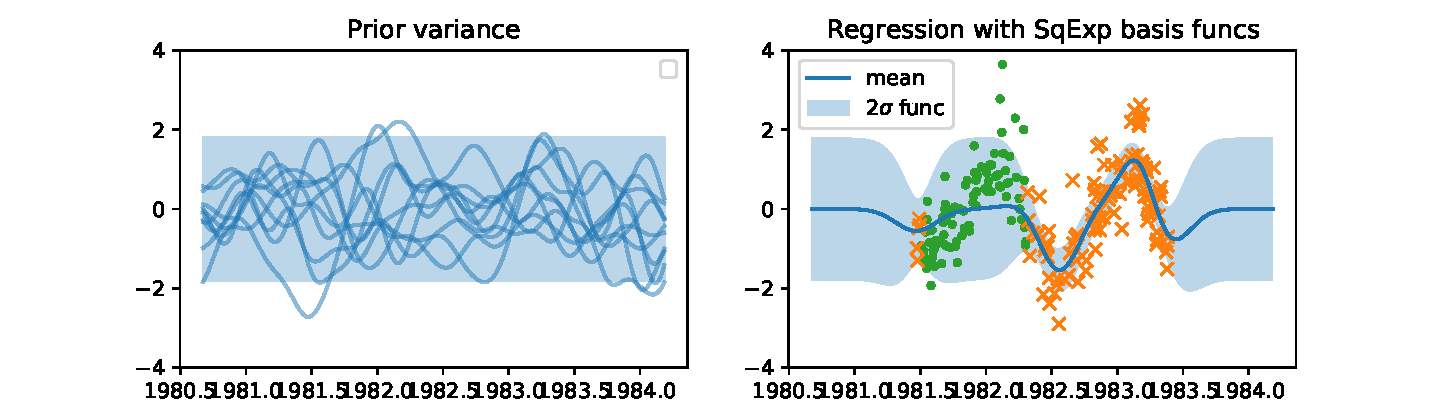
\includegraphics[width=\hsize,trim=2.2cm 0 2.2cm 0,clip]{./figures/gp/regression_basisfunc_prior_post_infinitebasis.pdf}
\end{figure}
\end{frame}


\begin{frame}{Recap}
What did we do?
\begin{enumerate}
\item Start with a basis function model.
\item \emph{Integrated out parameters} to directly find \emph{predictive distribution} $p(y_*|\vy)$.
\item Prediction only depended on \emph{inner products} of feature vectors.
\item We showed that we could compute inner products with a \emph{kernel function}.
\item Computational cost down from $\infty$ to $O(N^3)$.
\item Different \emph{representation} of a basis function model.
\end{enumerate} \pause

\vspace{0.4cm}

... but what is a Gaussian process?
\end{frame}


\begin{frame}{Priors on Function Values}
Another way of looking at our model:
\begin{gather}
p(y_n|f(\vx_n), \vx_n) = \NormDist{y_n; f(\vx_n), \sigma^2} \\
p(f(\mat X)) = \NormDist{f(\mat X); \vmu, \mat\Sigma}
\end{gather}
Remember: Each parameter \textit{implied} an entire function. So our prior placed a distribution on all the function values.

\vspace{0.4cm}

For a basis function model, find the prior on the vector of function values at each input point, denoted $f(\mat X)$, from the prior on the weights $p(\vtheta) = \NormDist{0, \mat I_M}$
\begin{gather}
% \vmu = \Exp{p(\vtheta)}{\Phi(\mat X)\vtheta} = \Phi(\mat X)\vmu_p \\
\mat\Sigma = \Var{p(\vtheta)}{\Phi(\mat X)\vtheta} = \Phi(\mat X)\Phi(\mat X)\transpose
\end{gather} \pause
A Gaussian process specifies $[\Phi(\mat X)\Phi(\mat X)\transpose]_{ij} = \vphi(\vx_i)\transpose\vphi(\vx_j) = k(\vx_i, \vx_j)$ \emph{directly}:
\begin{equation}
p(f(X)) = \NormDist{f(X); 0, k(\mat X, \mat X)}
\end{equation}
\end{frame}


\begin{frame}{So what really is a Gaussian process?}
See handwritten notes for:
\begin{itemize}
\item Definition of Gaussian process
\item Gaussian processes as distributions on functions
\item BLR defines a Gaussian process
\item Find the posterior of a GP
\end{itemize}
\end{frame}


% \begin{frame}{Gaussian Process Posterior}
% What is the posterior in a GP?
% \begin{itemize}
% \item Can't ask about parameters, there may be infinite number!
% \item Solution: Only ask questions about the function $f(\vx_*)$, or prediction $y_*$.
% \end{itemize}

% \vspace{0.3cm}

% \emph{Example}: Given $f \sim \mathcal{GP}(0, k(\cdot, \cdot'))$ and $p(y_n|f(\vx_n), \vx_n)$, \\
% find $p(f(\vx_*)|\vy, X)$. \pause
% Usual approach. Start with probability of everything (all relevant variables):
% \begin{align}
% p(f(\vx_*), f(X), \vy, X) = \frac{\colchar{$p(\vy|f(X)$}{green}, X)p(f(}{}
% \end{align}

% \end{frame}







% \begin{frame}{Exercises}
% Exercises:
% \begin{itemize}
% \item Find a cheap way to compute the value of the marginal likelihood of BLR. You will need to expand the density of the Gaussian.
% \item Using a GP prior with kernel $k(\vx, \vx')$, find the posterior for a new observation $p(y_*|\vy)$.
% \item What is the difference between the posterior on a new observation and the posterior on a function value?
% \item See exercises document for more exercises (materials).
% \end{itemize}
% \end{frame}


\begin{frame}{Recommended reading}
\begin{itemize}
\item \citet{gpml} \S 2.1 + \S 2.2
\end{itemize}
\end{frame}








%%%%%%%%%%%%%%%%%%%%%%%%%%%%%%%%%%%%%%%%%
% REFERENCES
%%%%%%%%%%%%%%%%%%%%%%%%%%%%%%%%%%%%%%%%%
\begin{frame}[t,allowframebreaks]
\frametitle{References}
\linespread{1.0}
\tiny
\bibliographystyle{apalike}
\bibliography{../includes/pi-literature}
\end{frame}



\end{document}
%%% Local Variables: 
%%% mode: latex
%%% TeX-master: t
%%% End: 
